\documentclass[12pt,twoside]{report}
\usepackage{float}
\usepackage{tikz}
\usepackage[siunitx]{circuitikz}
\usetikzlibrary{calc}    
\tikzset{
  dim above/.style={to path={\pgfextra{
        \pgfinterruptpath
        \draw[>=latex,|<->|] let
        \p1=($(\tikztostart)!2mm!90:(\tikztotarget)$),
        \p2=($(\tikztotarget)!2mm!-90:(\tikztostart)$)
        in(\p1) -- (\p2) node[pos=.5,sloped,above]{#1};
        \endpgfinterruptpath
      }(\tikztostart) -- (\tikztotarget) \tikztonodes
    }
  },
  dim below/.style={to path={\pgfextra{
        \pgfinterruptpath
        \draw[>=latex,|<->|] let 
        \p1=($(\tikztostart)!2mm!90:(\tikztotarget)$),
        \p2=($(\tikztotarget)!2mm!-90:(\tikztostart)$)
        in (\p1) -- (\p2) node[pos=.5,sloped,below]{#1};
        \endpgfinterruptpath
      }(\tikztostart) -- (\tikztotarget) \tikztonodes
    }
  },
}

\usepackage{graphicx}																		
\usepackage[romanian]{babel}
\usepackage[unicode]{hyperref} 
\usepackage{amsmath,epsfig,pifont,calc,pifont,pstricks}
\usepackage{rom}
\usepackage{color}
\usepackage{listings}
\definecolor{mygreen}{RGB}{28,172,0}
\definecolor{mylilas}{RGB}{170,55,241}
	

%%% setari ale paginii
%indentarea la inceput de paragraf
\setlength{\parindent}{3ex}

%dimensiunea textului pe pagina
\setlength{\voffset}{-2cm}
\setlength{\textheight}{23cm}  
\setlength{\textwidth}{16cm}
\setlength{\topmargin}{0cm}
\setlength{\headsep}{1cm}
\renewcommand{\baselinestretch}{1.2}
\newcommand{\myindent}{\hspace*{3ex}}
%\renewcommand{\baselinestretch}{1}

%margini
\setlength{\oddsidemargin}{0.5cm}
\setlength{\evensidemargin}{-0.3cm}
%\raggedright
\raggedbottom

%% begin preambul - macro-uri definite de autor
\newcommand{\D}{\mathrm{d}}	% va fi folosita in mediul matematic, pentru diferentiala d
\newcommand{\I}{\mathrm{i}}	% va fi folosita in mediul matematic, pentru unitatea imaginara
\newcommand{\eul}{\mathrm{e}}	% numarul lui Euler
\newcommand{\vect}[1]{\mathbf{#1}}	% comanda cu un argument, pentru scrierea vectorilor cu lidere aldine, drepte
                                    % comanda \vec a LaTeX pune sageti deasupra.
																										
\newcommand{\reale}{\mbox{${\scriptstyle \rm I\!R}$}}  % multimea numerelor reale
\newcommand{\complexe}{\mbox{${\scriptstyle \rm I\!\!\!\!C}$}}
\newcommand{\rationale}{\mbox{${\scriptstyle \rm I\!\!\!\!Q}$}}
\newcommand{\naturale}{\mbox{${\scriptstyle \rm I\!\!N}$}}
\newcommand{\intregi}{\mbox{${\scriptstyle \rm Z\!\!\!Z}$}}

\makeatletter
\setlength{\@fptop}{0pt}
\makeatother

\begin{document}
\title{\LARGE{\textbf{Proiectarea Algoritmilor} \\Tema 0\\}}
\author{Facultatea de Automatic'a 'si Calculatoare\\Universitatea Politehnic'a Bucure'sti\\\\ {\em Du'tu Alin C'alin}}
\maketitle
\newpage
\tableofcontents
\newpage
\chapter{Introducere}
\section{Descrierea problemei rezolvate 'si specificarea solu'tiilor alese}
Problema aleas'a este cea a analizei opera'tiilor unor structuri de date abstracte. Structurile alese fac parte din categoria cozilor de prioritate, astfel s-au ales pentru compara'tie arborele AVL 'si Max-Heap-ul 'si se vor compara prin utilizarea opera'tiilor comune acestora.
\newline 
\myindent
AVL tree este un arbore binar de c'autare care are proprietatea de auto-echilibare ce 'ii permite s'a execute opera'tiile unui arbore binar de c'autare obi'snuit mult mai eficient. Pentru AVL se iau 'in vedere opera'tiile de creare a structurii, ad'augare a unui element, opera'tiile de rota'tie st'anga 'si rota'tie dreapta, g'asirea elementului maxim 'si minim, eliminarea elementului maxim 'si a celui minim din structur'a 'si 'stergerea structurii. Max-Heap-ul este o structur'a de date bazat'a pe un arbore complet cu proprietatea c'a nodul cu valoarea maxim'a se gase'ste chiar 'in r'ad'acin'a. Pentru Max - Heap se vor implementa opera'tiile de creare a structurii, ad'augare a unui element, g'asirea elementului maxim, swift Up si swift Down, extragerea elementului maxim 'si 'stergerea structurii.
\vspace{5 mm}
\section{Specificarea criteriilor de evaluare}
Pentru evaluarea structurilor se vor folosi teste variate, cresc'atoare, descresc'atoare 'si generate random folosind un instrument online de generare a numerelor in ordine aleatoare\cite{Random} at'at pentru AVL c'at 'si pentru Max - Heap. Principalele criterii de evaluare luate 'in calcul pentru ambele structuri sunt timpii de execu'tie care vor testa rapiditatea structurilor pentru diferite input-uri, calculul complexit'a'tilor 'si dificulatatea implement'arii structurii propriu-zise.
\section{Exemple de aplica'tii practice pentru problema aleas'a}
Av\^and 'in vedere propriet'a'tile AVL-ului fa't'a de alte structuri cum ar fi Arborii Ro'su - Negru se poate constata c'a AVL-ul nu mai este foarte folosit in practic'a deoarece exist'a structuri mult mai eficiente, 'insa un exemplu care ar fi perfect pentru folosirea acestei structuri este gestionarea datelor pentru inventarul trenurilor dintr-o re'tea feroviar'a deoarece exemplul se bazeaz'a pe necesitatea c'aut'arii unui tren 'in func'tie de greutate sau de inventar 'si nu necesit'a foarte multe inser'ari 'si 'stergeri de obiecte. Max heap-ul are avantajul de a avea nodul cel mai mare 'in r'ad'acin'a 'si de aceea am putea avea ca exemplu de aplica'tie gestionarea pacien'tior dintr-un centru de analize 'in functie de prioritatea lor 'intruc\^at se poate afla foarte repede care va fi urm'atorul pacient. Aceste dou'a exemple au fost implementate suplimentar pe l\^ang'a testele pentru opera'tii 'si vor oferi informa'tii dintr-o prespectiv'a practic'a care vor contribui la compararea structurilor.
\chapter{Prezentarea Solu'tiilor}
Pentru acest proiect s-au implementat structurile de arbore AVL 'si Max-heap. Pentru ambele structuri s-a urm'arit, 'in principiu, comportamentul opera'tiilor de: creare a structurii, ad'augare a unui element, g'asierea elementului maxim, extragerea elementului maxim sau 'stergerea elementului maxim din structur'a 'si 'stergerea structurii.
\section{Descrierea modului 'in care functioneaz'a algoritmii}
\subsection{AVL Tree}
Arborele AVL este un arbore binar de c'autare care are 'in plus proprietatea de auto-echilibrare. Aceast'a proprietate se refer'a la faptul c'a diferen'ta 'in'al'timii subarborelui st\^ang cu 'in'al'timea suboarborelui drept nu poate fi mai mare de un nod. Dac'a aceast'a condi'tie este 'inc'alcat'a atunci arborele va fi reechilibrat pentru a se p'astra proprietatea de echilibru\cite{SD}.
\vspace{5 mm}
\newline
\myindent
O alt'a proprietate a arborelui AVL este factorul de balan't'a care este egal pentru oricare nod din arbore cu diferen'ta dintre 'in'al'timea subarborelui st\^ang 'si 'in'al'timea subarborelui drept si poate lua valorile {-1, 0 ,1}, -1 pentru un AVL left-heavy, 0 pentru un AVL echilibrat 'si 1 pentru un AVL right-heavy\cite{SD}.
\vspace{5 mm}
\newline
\myindent
Pentru implementarea algoritmilor s-au folosit diferite surse de inspira'tie pentru implementarea structurii propriu-zise 'si pentru implementarea opera'tiilor acestuia, dar si cuno'stin'tele dob\^andite p\^an'a acum la cursurile de Structuri de date incluz\^and cursurile 'si laboratoarele parcurse\cite{GeeksforGeeks, SD}. Implementarea acestei structuri cuprinde doar nodul r'ad'acin'a. La 'inceput s-a optat 'si pentru implementarea cu santinel'a nil, ins'a pentru u'surin't'a s-a renun'tat la aceast'a variant'a. Implementarea opera'tiilor este in mare parte iterativ'a cu excep'tia opera'tiilor de inserare 'si eliminare de elemente care sunt recursive.
\vspace{5 mm}
\newline
\myindent
Pentru verificarea opera'tiilor de inserare a unui element 'si de g'asire a maximului respectiv minimului din structur'a s-a folosit func'tia Inorder care afi'seaz'a 'in fi'sierul de output toate nodurile arborelui Inorder. 'In plus s-au ad'augat 'in fi'sier 'si rezulatele opera'tiilor de g'asire a maximului 'si minimului, pentru comparare cu rezultatul functiei Inorder demonstr\^and astfel corectitudinea opera'tiei. Pentru opera'tia de 'stergere se mai afi'seaz'a inca odat'a noile valori extreme 'si se verific'a tot cu rezultatul functiei Inorder. De asemenea, pentru testarea inser'arii am folosit un instrument online care mi-a permis s'a verific arborele structura arborelui\cite{AVLVisualization}.
\vspace{5 mm}
\subsection{Max - Heap}
Max-heap-ul este un arbore binar complet cu proprietatea c'a: pentru orice nod, cheia nodului este mai mare decât cheile din nodurile copii, dacă există copii \cite{SD}.
\newline
\myindent
Pentru implementarea Heap-ului s-au folosit 'in principal cuno'stin'tele acumulate, dar 'si laboratoarele f'acute la cursul de Structuri de Date\cite{SD}. Toate opera'tiile implementate sunt iterative. 
\newline
\myindent
Pentru verificarea inser'arii s-a folosit un instrument de vizualizare\cite{HeapVisualization} cu care se poate vedea aranjarea elementelor pe Heap. Pentru maxim s-a folosit un instrument online care s'a afi'seze maximul dintr-o list'a de numere, 'in acest caz din input\cite{MaxTool}. Iar pentru delete s-a efectuat aceea'si verificare ca la maxim cu precizarea c'a s-a eliminat vechiul maxim din list'a.
\vspace{5 mm}
\section{Analiza complexit'a'tii solu'tiilor}
\subsection{AVL Tree}
Conform teoriei un arbore AVL are 'in'al'timea O(log n). Urmeaz'a s'a fie demonstrat'a aceast'a afirma'tie. Fie h, 'in'al'timea arborelui 'si T(H) num'arul minim de noduri cu 'in'al'timea h. Pornim de la premisa c'a: Dac'a subarborele st'ang este umplut p\^an'a la 'in'al'timea h-1, atunci subarborele drept trebuie umplut p\^an'a la 'in'al'timea h-2. Astfel num'arul minim de noduri cu 'in'al'timea h este:
\newline
$T(h)$ = $T(h - 1)$ + $T(h - 2)$ + 1; cu $T(0)$ = 1, $ T(1)$ = 2 \\
$T(h - 1)$ = $T(h - 2)$ + $T(h - 3)$ + 1 $\Rightarrow$ T(h) = 2 *  $T(h - 2)$ + $T(h - 3)$ + 2\\
$T(h - 2)$ = $T(h - 3)$ + $T(h - 4)$ + 1 $\Rightarrow$ T(h) = 3 *  $T(h - 3)$ + $T(h - 4)$ + 2\\
...
De unde rezult'a c'a $T(h)$ = h * $T(h - h) + (h - 1) * $T(h - h + 1) + $2^{h}$ = 3h - 2 + $2^{h}$ $\Rightarrow$ $T(h)$  $>$ $2^{h}$\\
$\Rightarrow$  $log$ $T(h)$ $>$ h. Fie $T(h) = n$, unde n este num'arul de noduri $\Rightarrow$ $log$ $n$ $>$ h $\Rightarrow$ $h$ = $O(log$ $n)$
\vspace{5 mm}
\subsubsection{Create AVL}
Crearea unui AVL gol este o opera'tie foarte simpl'a f'ar'a apeluri recursive, f'ar'a structuri repetitive 'si care con'tine instructiuni de complexitate O(1), deci crearea arborelui AVL 'in cel mai r'au caz are complexitatea O(1).
\vspace{5 mm}
\subsubsection{Rotate left \& Rotate right}
Opera'tiile de rotire ale nodurilor sunt necesare pentru echilibrarea arborelui 'in cazul 'in care factorul de balan't'a este mai mare dec\^at 1 sau mai mic dec\^at -1. De asemeneta, rotirea propriu-zis'a este o opera'tie care nu necesit'a recuren'te sau bucle repetitive, deci in cel mai r'au caz rotirea fie ea st\^ang'a sau dreapt'a are complexitatea O(1).
\vspace{5 mm}
\subsubsection{Insert}
Inserarea unui nod are trei etape: prima reprezint'a crearea nodului care are complexitate O(1) deoarece opera'tia se execut'a iterativ 'si f'ar'a structuri repetitive, a doua etap'a const'a 'in gasirea locului unde trebuie ad'augat nodul. 'In worst case, se parcurge arborele pe toata 'inal'timea lui, asta 'insemn\^and complexitatea O(log n) 'si apoi urmeaz'a reechilibrarea arborelui, opera'tie ce are complexitatea in cel mai r'au caz tot O(log n), deoarece ajungand la frunze algoritmul se intoarce 'si face rotirile necesare pentru echilibrare (O(1)) de la frunz'a p\^an'a la r'ad'acin'a, practic o parcurgere invers'a a arborelui care are complexitate O(log n). Astfel Insert-ul ar avea complexitatea O(2 * log  n) = O(log n).
\vspace{5 mm}
\subsubsection{Get Min \& Max}
Pentru elementul minim 'si maxim se 'stie din teorie c'a ele se g'asesc la extremit'a'tile arborelui, 'in sensul c'a nodul minim este frunza cea mai din st\^anga, iar nodul maxim este frunza cea mai din dreapta. Deci, pentru g'asirea fie a minimului, fie a maximului este necesar'a o parcurgere pe toat'a 'in'al'timea arborelui care are complexitatea O(log n). Astfel complexitatea opera'tiei de g'asire a minimului 'si maximului dintr-un AVL este  O(2 * log  n) = O(log n).
\vspace{5 mm}
\subsubsection{Delete}
Opera'tia de 'stergere a unui element, desi este mai complex'a fa't'a de inserare, ea are aceea'si complexitate. Motivul este c'a opera'tia incepe prin c'autarea nodului de eliminat ( in worst case O(log n)), apoi inlocuirea nodului eliminat care are 3 cazuri: C\^and nodul eliminat nu are copii 'si atunci opera'tia are complexitatea O(1), c\^and are un copil 'si atunci opera'tia are complexitatea tot O(1) 'si c\^and are 2 copii, caz 'in care se poate alege fie valoarea maxim'a din subarborele st\^ang, fie valorea minim'a din subarborele drept ( in aceast'a implementare s-a luat 'in considerare valoarea maxim'a din subarborele st\^ang). Acest caz are complexitatea O(log n) deoarece se parcurge arborele p\^an'a la frunze. Ultima etap'a a opera'tiei este reechilibrarea arborelui (O(log n)). 'In total avem complexitatea O(3 * log n) = O(log n).
\vspace{5 mm}
\subsection{Max-Heap}
\subsubsection{Create Heap}
Opera'tia de creare a Heap-ului nu are bucle repetitive sau recursivit'a'ti, de aceea complexitatea opera'tiei este O(1).
\vspace{5 mm}
\subsubsection{Sift Up \& Sift Down}
Opera'tia de Sift Up 'in aceast'a implementare nu este recursiv'a si nu are blocuri repetitive, deci complexitatea este O(1). 'In schimb Sift Down in cel mai r'au caz duce nodul r'ad'acin'a p\^an'a la frunze, practic o parcurgere a arborelui, deci complexitatea este O(h), unde h este 'in'al'timea arborelui, ins'a dat fiind faptul c'a 'in teorie se spune c'a heap-ul este un arbore complet se poate afirma c'a O(log n) este complexitatea opera'tiei de Sift Down.
\vspace{5 mm}
\subsubsection{Insert}
'In cel mai r'au caz arborele adaug'a un nod la frunze si dup'a se face sift up p\^an'a c\^and nodul nou ajunge la r'ad'acin'a. Stiind c'a complexitatea lui Sift Up este O(1) se deduce c'a insertul este echivalent 'in acest caz cu parcurgerea arborelui de sus 'in jos ceea ce 'inseamn'a complexitate O(log n). Deci insertul are complexitatea O(log n).
\vspace{5 mm}
\subsubsection{Get Max}
Stiind c'a valoarea maxim'a se g'ase'ste la r'ad'acin'a rezult'a complexitate O(1), deci complexitatea g'asirii elementului maxim este O(1).
\vspace{5 mm}
\subsubsection{Extract Max}
Pentru Extract Max, opera'tia propriu-zis'a de extragere este echivalent'a cu opera'tia Get Max care are complexitatea O(1) 'impreun'a cu opera'tia de Sift Down care mai adaug'a complexitatea O(log n). Deci, complexitatea opera'tiei de extragere a elementului maxim 'in cazul cel mai nefavorabil este O(log n + 1) = O(log n).
\section{Avantaje 'si dezavantaje}
Principalele avantajele ale structurilor AVL Tree 'si Max-Heap sunt rapiditatea opera'tiilor de inserare, c'autare 'si g'asire a maximului, dar 'si eliminarea maximului deoarece toate aceste opera'tii au complexitate O(log n) care este mult mai bun'a fa'ta de complexit'a'tea unui arbore binar de c'autare obi'snuit de exemplu 'si ofer'a mai mult'a flexibilitate. Principalul dezavantaj pentru AVL este dificultatea implement'arii codului pentru opera'tii, iar pentru Max-Heap  principalul dezavantaj ar fi organizarea memoriei.



\chapter{Evaluare}
\section{Modalitatea de construire a testelor}
Pentru evaluarea opera'tiilor structurilor de AVL Tree 'si Max - Heap s-au implementat 'in etapa trecut'a c\^ate 5 teste care au fost construite folosind un generator de numere distincte\cite{Random} 'si un instrument de sortare online\cite{Endmemo}, numerele fiind generate 'intr-o ordine aleatoare 'si mai mici de 1000. Aceste teste au un num'ar de 5, 10, 25, 50 'si 100 de elemente distincte. Pentru o mai bun'a acurate'te a performan'tei opera'tiilor se vor mai ad'auga un set de 5 teste pentru fiecare structur'a. Un test va fi de 250 de elemente generate 'in ordine aleatoare, dou'a teste vor fi de 500 'si 1000 de elemente 'si vor fi generate descresc'ator, iar celelalte dou'a teste vor fi de 5000 'si 10000 de elemente generate cresc'ator.
\myindent Fiecare test va rula toate opera'tiile structurii de date reprezentate. Pentru AVL se vor executa: Crearea structurii, Inserarea elementelor, C'autarea maximului 'si minimului, Eliminarea maximului 'si minimului din structur'a 'si 'Stergerea structurii, iar pentru Heap se vor executa: Crearea structurii, Inserarea elementelor, Preluarea nodului cu valoare maxim'a, Extrgerea nodului cu valoare maxim'a 'si 'stergerea structurii.
\vspace{5 mm}
\section{Rezultatele testelor}
\begin{table}[ht]
\centering
\caption{Timpii de execu'tie pentru crearea structurilor}
\begin{tabular}{| p{5cm} | p{5cm} | p{5cm} |}
\hline
N & AVL Tree & Max - Heap \\
\hline\hline
5 & 0.001178 ms & 0.001106 ms \\
\hline
10 & 0.000726 ms & 0.001051 ms \\
\hline
25 & 0.000682 ms & 0.000986 ms \\
\hline
50 & 0.000677 ms & 0.00114 ms \\
\hline
100 & 0.000676 ms & 0.002253 ms \\
\hline
250 & 0.000707 ms & 0.003481 ms \\
\hline
500 & 0.000898 ms & 0.005623 ms \\
\hline
1000 & 0.000984 ms & 0.010363 ms \\
\hline
5000 & 0.000797 ms & 0.04761 ms \\
\hline
10000 & 0.000861 ms & 0.362846 ms \\
\hline
\end{tabular}
\end{table}
\FloatBarrier

\begin{figure}[ht]
\centering
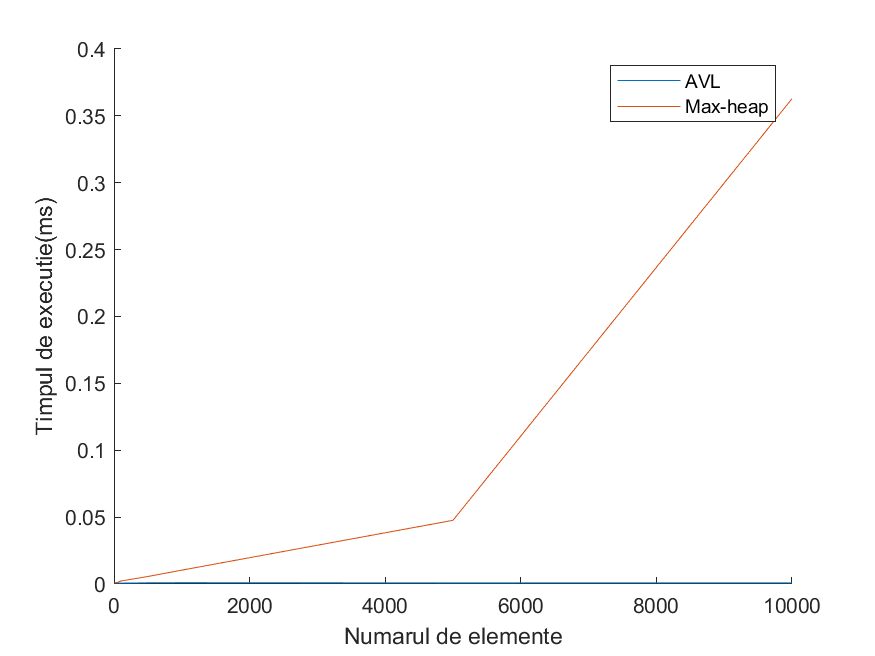
\includegraphics[scale=0.8]{Fisiere/creare}
\caption {Diagrama pentru crearea structurilor}
\end{figure}
\FloatBarrier

\begin{table}[ht]
\centering
\caption{Timpii de execu'tie pentru inserarea elementelor}
\begin{tabular}{| p{5cm} | p{5cm} | p{5cm} |}
\hline
N & AVL Tree & Max - Heap \\
\hline\hline
5 & 0.001159 ms & 0.010295 ms \\
\hline
10 & 0.017719 ms & 0.010691 ms \\
\hline
25 & 0.041883 ms & 0.02151 ms \\
\hline
50 & 0.096804 ms & 0.052967 ms \\
\hline
100 & 0.221705 ms & 0.109183 ms \\
\hline
250 & 0.591891 ms & 0.225686 ms \\
\hline
500 & 1.29952 ms & 0.379961 ms \\
\hline
1000 & 3.05291 ms & 0.692936 ms \\
\hline
5000 & 19.6206 ms & 11.6697 ms \\
\hline
10000 & 59.8021 ms & 24.26 ms \\
\hline
\end{tabular}
\end{table}
\FloatBarrier

\begin{figure}[ht]
\centering
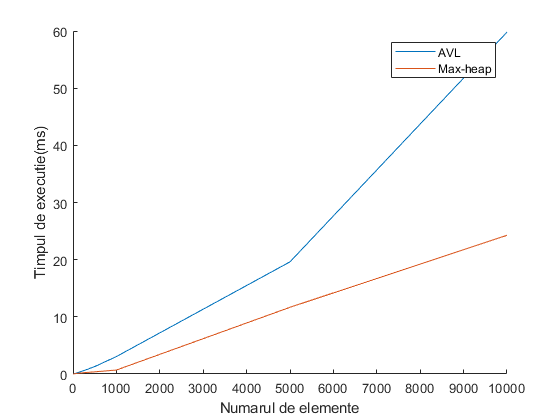
\includegraphics[scale=0.8]{Fisiere/inserare}
\caption {Diagrama pentru inserarea elementelor}
\end{figure}
\FloatBarrier

\vspace{5 mm}
\begin{table}[ht]
\centering
\caption{Timpii de execu'tie pentru g'asirea elementelor maxime}
\begin{tabular}{| p{5cm} | p{5cm} | p{5cm} |}
\hline
N & AVL Tree & Max - Heap \\
\hline\hline
5 & 0.007937 ms & 0.000431 ms \\
\hline
10 & 0.008015 ms & 0.000409 ms \\
\hline
25 & 0.008226 ms & 0.000412 ms \\
\hline
50 & 0.008193 ms & 0.000427 ms \\
\hline
100 & 0.008362 ms & 0.00044 ms \\
\hline
250 & 0.008447 ms & 0.000453 ms \\
\hline
500 & 0.010743 ms & 0.000468 ms \\
\hline
1000 & 0.01005 ms & 0.000466 ms \\
\hline
5000 & 0.011588 ms & 0.000485 ms \\
\hline
10000 & 0.012177 ms & 0.000631 ms \\
\hline
\end{tabular}
\end{table}
\FloatBarrier

\begin{figure}[ht]
\centering
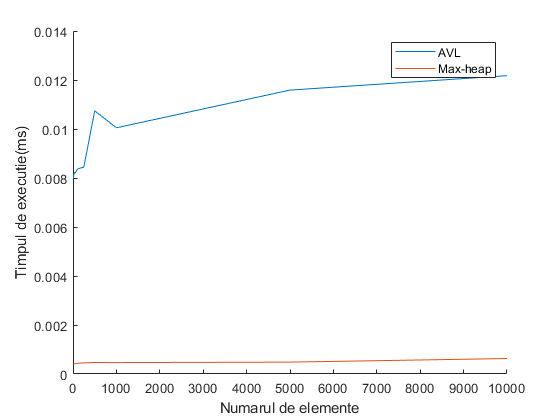
\includegraphics[scale=0.8]{Fisiere/FindMax}
\caption {Diagrama pentru g'asirea elementelor maxime}
\end{figure}
\FloatBarrier

\vspace{5 mm}
\begin{table}[ht]
\centering
\caption{Timpii de execu'tie pentru eliminarea elementelor maxime}
\begin{tabular}{| p{5cm} | p{5cm} | p{5cm} |}
\hline
N & AVL Tree & Max - Heap \\
\hline\hline
5 & 0.000388 ms & 0.000667 ms \\
\hline
10 & 0.000677 ms & 0.000737 ms \\
\hline
25 & 0.000573 ms & 0.001418 ms \\
\hline
50 & 0.000555 ms & 0.001529 ms \\
\hline
100 & 0.00108 ms & 0.001674 ms \\
\hline
250 & 0.001119 ms & 0.001795 ms \\
\hline
500 & 0.000832 ms & 0.001991 ms \\
\hline
1000 & 0.000983 ms & 0.002041 ms \\
\hline
5000 & 0.005285 ms & 0.00266 ms \\
\hline
10000 & 0.00594 ms & 0.002867 ms \\
\hline
\end{tabular}
\end{table}
\FloatBarrier

\begin{figure}[ht]
\centering
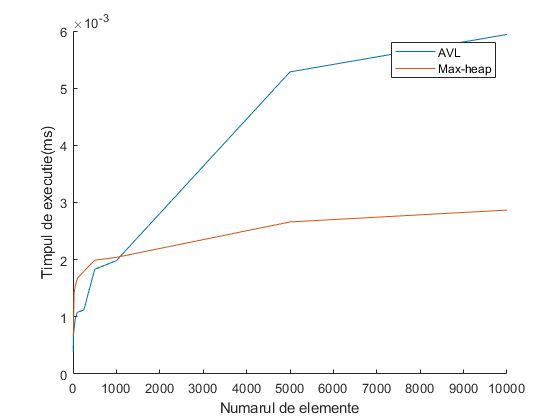
\includegraphics[scale=0.8]{Fisiere/DelMax}
\caption {Diagrama pentru eliminarea elementelor maxime}
\end{figure}
\FloatBarrier

\begin{table}[ht]
\centering
\caption{Timpii de execu'tie pentru 'stergerea structurii}
\begin{tabular}{| p{5cm} | p{5cm} | p{5cm} |}
\hline
N & AVL Tree & Max - Heap \\
\hline\hline
5 & 0.000501 ms & 0.000473 ms \\
\hline
10 & 0.000808 ms & 0.000328 ms \\
\hline
25 & 0.001794 ms & 0.000268 ms \\
\hline
50 & 0.003458 ms & 0.000297 ms \\
\hline
100 & 0.007003 ms & 0.000362 ms \\
\hline
250 & 0.013364 ms & 0.000416 ms \\
\hline
500 & 0.02463 ms & 0.000444 ms \\
\hline
1000 & 0.04781 ms & 0.00032 ms \\
\hline
5000 & 0.369463 ms & 0.00076 ms \\
\hline
10000 & 0.753662 ms & 0.00088 ms \\
\hline
\end{tabular}
\end{table}
\FloatBarrier

\begin{figure}[ht]
\centering
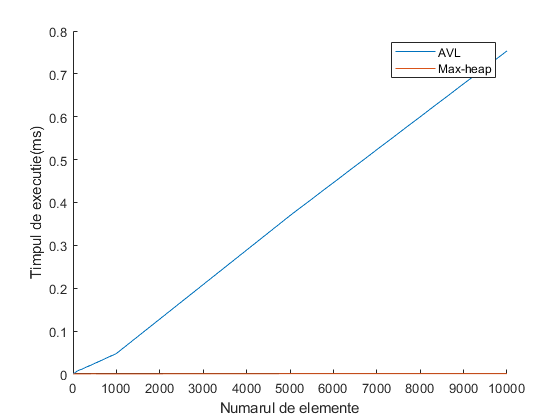
\includegraphics[scale=0.8]{Fisiere/Del}
\caption {Diagrama pentru 'stergerea structurilor}
\end{figure}
\FloatBarrier

\section{Prezentarea rezultatelor testelor}
Pentru crearea structurii propriu-zise se poate observa c'a AVL-ul are pentru orice set de date o eficien't'a mult mai bun'a din punctul de vedere al timpului de execu'tie fa't'a de Max-Heap, 'ins'a diferen'ta nu este foarte mare. Pentru Insert pentru teste sub 1000 de elemente structurile sunt la fel de eficiente, ins'a pentru teste mai mari Max - Heap - ul este mult mai bun fa't'a de AVL. Pentru g'asirea elementului maxim Max-Heap-ul av\^and valoarea maxim'a in nodul r'ad'acin'a este clar c'a v'a scoate timpi foarte mici de execu'tie datorit'a complexit'a'tii O(1) care 'in compara'tie cu O(log n) este diferen't'a semnificativ'a in special la seturi foarte mari de date. Pentru eliminarea elementului maxim AVL-ul este mai eficient dec\^at Max Heap-ul pentru input-uri mai mici de 1200 de elemente, 'insa pentru testele mai mari Max-Heap-ul este mai bun. 'In final, pentru 'stergerea structurilor, Max-Heap-ul are o performan't'a mult mai bun'a 'in compara'tie cu AVL.

\section{Specifica'tiile sistemului de calcul}
Tema a fost implementat'a folosind C++, compilat'a folosind G++ versiunea 9.3.0 'si a fost rulat'a pe o masin'a virtual'a cu Ubuntu 20.04 cu 6GB RAM aloca'ti. Configura'tia host-ului este Windows 10 cu Procesor Intel Core i7-5500U cu 2 core-uri de 2,4 GHZ, 16 GB RAM 'si plac'a Video NVidia cu 2GB.

\vspace{5 mm}
\nocite{*}
\bibliographystyle{plainrom}
\addcontentsline{toc}{chapter}{Bibliografie}
\bibliography{Bibliografie}
\end{document}